% Assignment 3 -- Argumentation Engine and Strategic Argumentation
% Compile with:  pdflatex report.tex  (run twice for the table of contents / references)
% Needs a standard TeX Live / MiKTeX install (packages: geometry, amsmath, amssymb, booktabs,
% tabularx, enumitem, hyperref, xcolor, pgfplots).
\documentclass[11pt,a4paper]{article}

\usepackage[T1]{fontenc}
\usepackage[utf8]{inputenc}
\usepackage{lmodern}
\usepackage[margin=2.4cm]{geometry}
\usepackage{amsmath,amssymb}
\usepackage{booktabs}
\usepackage{tabularx}
\usepackage{enumitem}
\usepackage{xcolor}
\usepackage{pgfplots}
\pgfplotsset{compat=1.16}
\usepackage[colorlinks=true,linkcolor=blue!50!black,urlcolor=blue!50!black]{hyperref}

\setlength{\parindent}{0pt}
\setlength{\parskip}{0.55em}
\setlist{itemsep=0.2em,topsep=0.3em}
\renewcommand{\arraystretch}{1.15}

% inline code (works for names containing underscores outside of section titles)
\newcommand{\code}[1]{\texttt{\detokenize{#1}}}
\newcommand{\defeats}{\rightharpoonup}
\newcommand{\indirect}{\rightsquigarrow}
\newcommand{\Ai}{A_i}
\newcommand{\In}{\textsf{in}}
\newcommand{\Out}{\textsf{out}}
\newcommand{\Undec}{\textsf{undec}}

\title{\textbf{Assignment 3: Argumentation Engine\\and Strategic Argumentation}\\[0.3em]
\large Grounded direct argumentation mechanism, Theorems 5.3 and 5.4}
\author{Autonomous Systems, 4th Year\\[0.8em]
\textbf{Group Members}\\[0.3em]
\begin{tabular}{ll}
\toprule
\textbf{Name} & \textbf{Roll Number}\\
\midrule
Om Chandra Sharma & B23CS1048\\
Mayank Dahiya & B23CS1035\\
Anmol Yadav & B23CS1004\\
Rudra Gupta & B23CS1098\\
\bottomrule
\end{tabular}}
\date{\today}

\begin{document}
\maketitle
\tableofcontents
\bigskip

\noindent All numbers in this report come from \code{python experiments.py} (seed 2024; output in
\code{results/}) and from \code{python -m unittest test_engine test_book_examples}.
Implementation: pure Python~3, no third-party packages.

%% ------------------------------------------------------------------ %%
\section{Overview of the deliverables}

\begin{tabularx}{\textwidth}{@{}lX@{}}
\toprule
File & Contents\\
\midrule
\code{argumentation.py} & Part 1: framework class and all engine functions\\
\code{strategic.py} & Part 2: mechanism, best responses, Theorem 5.3 check, Theorem 5.4 condition\\
\code{book_examples.py} & Figures 5.1--5.3 and Examples 5.10/5.11 of the textbook as objects\\
\code{experiments.py} & Random-instance experiment (writes \code{results/})\\
\code{test_engine.py}, \code{test_book_examples.py} & 48 unit and property tests\\
\code{demo.py}, \code{demo_output.txt} & Demonstration script and its captured output\\
\code{README.md}, this report & Documentation\\
\bottomrule
\end{tabularx}

%% ------------------------------------------------------------------ %%
\section{Part 1 -- The argumentation engine}

\code{argumentation.py} implements every requested function as a direct reading of the definitions.

\begin{itemize}
\item \textbf{Framework class.} \code{ArgumentationFramework(arguments, attacks)} stores the frozen argument set and the
  attack relation, validates that attacks only mention known arguments, and precomputes attackers and targets.
  Self-attacks are allowed. \code{parse("a->b, b<->c, d")} builds frameworks in one line.
\item \textbf{Basic notions.} $S$ is conflict-free iff no member of $S$ attacks a member of $S$; $S$ defends $a$ iff every
  attacker of $a$ is attacked by a member of $S$; $F(S)=\{a : S \text{ defends } a\}$; $S$ is admissible iff it is
  conflict-free and $S\subseteq F(S)$; $S$ is complete iff it is admissible and $F(S)\subseteq S$.
\item \textbf{Grounded} extension: least fixed point of $F$, obtained by iterating $F$ from $\emptyset$.
  \textbf{Complete} extensions: enumeration of subsets (only supersets of the grounded extension without self-attackers need
  be tried). \textbf{Preferred}: $\subseteq$-maximal admissible sets. \textbf{Stable}: conflict-free sets attacking every
  argument outside them. \textbf{Semi-stable}: complete extensions whose range $S\cup S^{+}$ is $\subseteq$-maximal.
\item \textbf{Labellings.} All $3^n$ labellings are generated and filtered with Caminada's conditions
  ($\In$ iff all attackers $\Out$; $\Out$ iff some attacker $\In$; $\Undec$ otherwise).
\item \textbf{Acceptance status} (preferred semantics by default): in every extension $\Rightarrow$ skeptically accepted;
  in some but not all $\Rightarrow$ credulously accepted; in none $\Rightarrow$ rejected.
\end{itemize}

\subsection{Tests on the book's examples}

The frameworks of Chapter~5 of the course textbook are encoded exactly as drawn
(\code{book_examples.py}); every value the book states is asserted in \code{test_book_examples.py}.
The graphs of Figures 5.1--5.3 were read off the book's drawings.

\begin{center}
\small
\begin{tabularx}{\textwidth}{@{}p{2.6cm}p{3.3cm}X@{}}
\toprule
Book example & Framework & Results reproduced by the engine\\
\midrule
Fig.\ 5.1, Ex.\ 5.5, 5.6, 5.8 &
$\alpha_3\!\to\!\alpha_2\!\to\!\alpha_1\!\leftarrow\!\alpha_4\!\leftarrow\!\alpha_5$ &
Admissible sets $\emptyset,\{3\},\{5\},\{3,5\},\{1,3,5\}$; $\{3,5\}$ defends 1 but is not complete;
$F(\emptyset)=\{3,5\}$, $F^2(\emptyset)=\{1,3,5\}$ = grounded; $\{1,3,5\}$ is the only complete (and preferred, stable,
semi-stable) extension; 1, 3, 5 skeptically accepted, 2, 4 rejected.\\[0.4em]
Fig.\ 5.2, Ex.\ 5.7, 5.8 &
$\alpha_1\leftrightarrow\alpha_2$, $\alpha_3$ alone &
Complete: $\{3\},\{1,3\},\{2,3\}$; grounded $\{3\}$; preferred $\{1,3\},\{2,3\}$; the three labellings $L^G$ (1, 2 undec),
$L_1$ (1 in, 2 out), $L_2$ (2 in, 1 out); Table 5.1's correspondence (grounded = minimal in, preferred = maximal in,
semi-stable = minimal undec, stable = no undec) verified; 3 skeptical, 1 and 2 credulous.\\[0.4em]
Fig.\ 5.3, Ex.\ 5.9 &
$b\!\to\!a$, $c\!\to\!b$, $d\!\to\!b$, $c\!\leftrightarrow\!d$, $e\!\to\!d$ &
Grounded $=\{a,c,e\}$ (as stated on p.~188); all other semantics coincide with it; $a,c,e$ skeptical, $b,d$ rejected.\\
\bottomrule
\end{tabularx}
\end{center}

Further frameworks (chain, odd cycle, self-attack, a case with preferred $\ne$ stable, Caminada's example with semi-stable
but no stable extensions) were derived by hand and are tested in \code{test_engine.py}. In addition, 300 random frameworks
are cross-checked against independent characterisations: complete extensions equal brute force over all subsets; legal
labellings are in bijection with complete extensions; grounded $=$ least complete $=\bigcap$ complete;
stable $\subseteq$ semi-stable $\subseteq$ preferred $\subseteq$ complete; preferred $=$ maximal complete. All 48 tests pass.

%% ------------------------------------------------------------------ %%
\section{Part 2 -- Grounded direct argumentation mechanism}

Agent $i$ owns a set $\Ai$ (the owners partition the arguments), reports a subset $R_i\subseteq \Ai$, and its utility is the
number of its own arguments in the grounded extension of the framework induced by $R_1\cup\dots\cup R_n$.
In \code{strategic.py}:

\begin{enumerate}
\item \code{grounded_direct_mechanism(attacks, reports)} induces the framework on the union of the reports (attacks with an
  unrevealed endpoint are dropped) and returns its grounded extension.
\item \code{best_responses(game, i, others_reports)} enumerates all $2^{|\Ai|}$ subsets (including $\emptyset$) and returns every
  report attaining the maximal utility.
\item \code{is_strategyproof(game)} (the property of Theorem 5.3) checks, for every agent and every combination of subsets the
  other agents could reveal, that revealing all of $\Ai$ attains the maximal utility, and returns all counterexamples.
  Outcomes are memoised on the union of the reports, so a full 3-agent check on 8 arguments takes milliseconds.
\item \code{satisfies_theorem_5_4(game)} checks that no agent owns two arguments $\alpha,\beta$ with an odd-length directed path
  $\alpha\indirect\beta$ in the full graph. Because the graph may contain cycles, paths are \emph{simple} (DFS with a visited
  set; \code{has_odd_simple_path}), the literal reading of ``directed path'' and the headline reading. I also implemented the
  \emph{walk} reading (\code{has_odd_walk}: BFS over (argument, parity) states, always terminating), where a self-loop or cycle
  can flip parity: $a\to x$, $x\to x$, $x\to b$ has an odd walk of length 3 though its only simple path has length 2. A switch
  decides whether $\alpha=\beta$ is allowed (odd cycle through $\alpha$, ``indirect self-defeat''), and another adds the
  book's conflict-freeness requirement. \textbf{Default: simple path, $\alpha\neq\beta$.}
\end{enumerate}

\paragraph{The book's statements.}
Theorem 5.3 (p.~200): the mechanism is strategyproof for acceptability maximisers iff for every agent $i$, every
$S\subseteq\Ai$ and every $A_{-i}$,
$|\Ai\cap E(\Ai\cup A_{-i})|\ \ge\ |\Ai\cap E((\Ai\setminus S)\cup A_{-i})|$; \code{is_strategyproof} checks exactly this, and the
test suite also transcribes the inequality literally and confirms that the two agree on 300 random games.
Theorem 5.4: if each agent's type is conflict-free \emph{and} contains no $\alpha_1,\alpha_2$ with $\alpha_1\indirect\alpha_2$
(odd-length path in the whole graph), the mechanism is strategyproof. The assignment words the condition as ``no two arguments
with an odd path''; the book additionally requires conflict-freeness, which between distinct arguments is an odd path of length~1
and otherwise only excludes self-attacks. \code{require_conflict_free=True} implements the book's exact wording and is reported
as a fifth reading below.

\subsection{The book's examples}

\paragraph{Example 5.10 / Fig.~5.4.} $x=\{1,4,5\}$, $y=\{2\}$, $z=\{3\}$, $R=\{(1,2),(2,3),(3,4),(3,5)\}$.
Truthfully the outcome is $\{1,3\}$, with utilities $u_x=1$, $u_y=0$, $u_z=1$.
\textbf{Misprint:} the book prints $u_y(o,\{3\})=1$ and $u_z(o,\{2\})=0$, i.e.\ with the two agents' argument sets exchanged;
the values above are the correct ones and are what the code computes. If $x$ withholds argument 1, the outcome is $\{2,4,5\}$ and
$u_x=2$, so the mechanism is not strategyproof; \code{best_responses} for $x$ returns exactly $\{4,5\}$. The checker finds
profitable deviations for $x$ only, matching the book's remark that for $y$ and $z$ truthful revelation weakly dominates revealing
nothing. The Theorem 5.4 condition is violated by $(x;1,4)$ and $(x;1,5)$, via the odd paths $1\to2\to3\to4$ and $1\to2\to3\to5$.

\paragraph{Example 5.11 / Fig.~5.5.} Add argument 6 (to $x$) and the defeat $(6,3)$. The truthful outcome is $\{1,4,5,6\}$, so $x$
gets all its arguments accepted and the checker confirms that truth-telling is dominant, although $1\indirect4$ and $1\indirect5$
still violate the Theorem 5.4 condition. This is the book's illustration that the condition is sufficient but not necessary.
\textbf{Misprint:} the discussion afterwards says argument~5 cancels the negative effect of the indirect defeat; it is
argument~\textbf{6}, which defeats 3, the argument that would otherwise defeat 4 and 5. The code confirms this: without 6 the
instance is manipulable again ($x$ gains by revealing $\{4,5\}$), while with 6 but without 5 it remains strategyproof; and 5
defeats nothing, so it cannot influence anyone else's status.

\paragraph{A further manipulable example.} Agent 0 owns $\{\alpha,\beta\}$, agent 1 owns $\{\delta\}$, attacks
$\alpha\leftrightarrow\delta$ and $\alpha\to\beta$. Truthfully all three arguments are undecided (utility 0). If agent 0 hides
$\alpha$, then $\delta$ and $\beta$ are unattacked and accepted (utility 1). The Theorem 5.4 condition is violated by
$(\alpha,\beta)$.

%% ------------------------------------------------------------------ %%
\section{Experiments}

\paragraph{Set-up.} For each attack probability $p\in\{0.1,0.2,\dots,0.9\}$ I drew \textbf{3000 random instances, 27\,000 in total}
(at least 1000 required): 6, 7 or 8 arguments (uniform); every ordered pair $(a,b)$, self-attacks $a\to a$ included, is an attack
with probability $p$; every argument is given to one of 3 agents uniformly (an agent may receive none). For each instance the
strategyproofness check is exhaustive (3 agents $\times$ all subsets of the agent's own arguments $\times$ all subset
combinations of the others), and Theorem 5.4's condition is evaluated under five readings: simple path / walk $\times$
$\alpha\ne\beta$ / $\alpha=\beta$ allowed, plus the book's exact wording (simple path, $\alpha\ne\beta$, types conflict-free).
The run takes about 4 minutes. With 3000 samples per $p$, each fraction has a 95\% confidence half-width of at most $\pm0.018$.
Per-instance records are in \code{results/instances.csv}.

\subsection{Fraction of strategyproof instances (question 1)}

\begin{center}
\small
\begin{tabular}{@{}rrrrrrr@{}}
\toprule
$p$ & \textbf{strategyproof} & \textbf{Thm 5.4 holds} & path, & walk, & walk, & book\\
    &                        & \textbf{(path, $\alpha\!\ne\!\beta$)} & $\alpha\!=\!\beta$ ok & $\alpha\!\ne\!\beta$ & $\alpha\!=\!\beta$ ok & wording\\
\midrule
0.1 & \textbf{0.744} & 0.241 & 0.120 & 0.221 & 0.120 & 0.121\\
0.2 & \textbf{0.374} & 0.053 & 0.012 & 0.033 & 0.012 & 0.012\\
0.3 & \textbf{0.170} & 0.012 & 0.002 & 0.004 & 0.002 & 0.002\\
0.4 & \textbf{0.108} & 0.002 & 0.000 & 0.000 & 0.000 & 0.000\\
0.5 & \textbf{0.089} & 0.000 & 0.000 & 0.000 & 0.000 & 0.000\\
0.6 & \textbf{0.113} & 0.000 & 0.000 & 0.000 & 0.000 & 0.000\\
0.7 & \textbf{0.166} & 0.000 & 0.000 & 0.000 & 0.000 & 0.000\\
0.8 & \textbf{0.284} & 0.000 & 0.000 & 0.000 & 0.000 & 0.000\\
0.9 & \textbf{0.528} & 0.000 & 0.000 & 0.000 & 0.000 & 0.000\\
\bottomrule
\end{tabular}
\end{center}

Overall 7725 of 27\,000 instances (28.6\%) are strategyproof.

\begin{center}
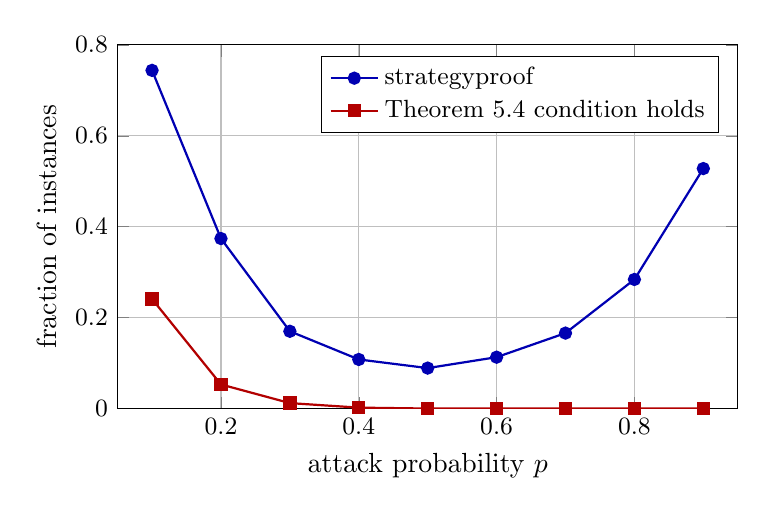
\begin{tikzpicture}
\begin{axis}[
  width=0.78\textwidth, height=6.2cm,
  xlabel={attack probability $p$}, ylabel={fraction of instances},
  xmin=0.05, xmax=0.95, ymin=0, ymax=0.8,
  grid=major, legend pos=north east, legend cell align=left,
  tick label style={font=\small}, legend style={font=\small}]
\addplot[blue!70!black, thick, mark=*] coordinates
  {(0.1,0.744) (0.2,0.374) (0.3,0.170) (0.4,0.108) (0.5,0.089) (0.6,0.113) (0.7,0.166) (0.8,0.284) (0.9,0.528)};
\addlegendentry{strategyproof}
\addplot[red!70!black, thick, mark=square*] coordinates
  {(0.1,0.241) (0.2,0.053) (0.3,0.012) (0.4,0.002) (0.5,0) (0.6,0) (0.7,0) (0.8,0) (0.9,0)};
\addlegendentry{Theorem 5.4 condition holds}
\end{axis}
\end{tikzpicture}

\small Strategyproof fraction and fraction satisfying the Theorem 5.4 condition (simple path, $\alpha\ne\beta$), by $p$.
\end{center}

\paragraph{Reading the curve.} Strategyproofness falls steeply from $p=0.1$ to $p\approx0.5$ and then \emph{rises} again. At low
$p$ the graph is sparse, so few arguments of the same agent are connected and there is little to gain by hiding. As $p$ grows,
attack chains and cycles connect an agent's arguments (more opportunities to profit from hiding), so the fraction drops. For
large $p$ the effect reverses because a self-attack has probability $p$, so about a fraction $p$ of the arguments attack
themselves. In a separate sample of 600 instances per $p$, the grounded extension of the full framework was empty in 94\%
($p=0.5$), 98\% ($p=0.6$) and about 100\% ($p\ge0.7$) of instances. When almost nothing can be accepted, utilities are mostly 0 for
every report and there is little to manipulate. The Theorem 5.4 condition is far more demanding than strategyproofness: it needs
\emph{every} pair of an agent's arguments to be free of odd paths, which is practically never true beyond $p\approx0.3$.

\subsection{Condition holds but the mechanism is manipulable (question 2)}

\begin{center}
\begin{tabular}{@{}lrrr@{}}
\toprule
Reading of the condition & holds & \dots and strategyproof & \dots but \textbf{not} strategyproof\\
\midrule
\textbf{simple path, $\alpha\ne\beta$ (headline)} & 928 & 928 & \textbf{0}\\
simple path, $\alpha=\beta$ allowed & 402 & 402 & \textbf{0}\\
walk, $\alpha\ne\beta$ & 777 & 777 & \textbf{0}\\
walk, $\alpha=\beta$ allowed & 402 & 402 & \textbf{0}\\
book wording (conflict-free types) & 405 & 405 & \textbf{0}\\
\bottomrule
\end{tabular}
\end{center}

\textbf{There are no such instances}: in 27\,000 instances and under every reading, whenever the odd-path condition holds
(including the book's exact wording), revealing everything is a best response against every combination of the others'
reports. This is exactly what Theorem 5.4 claims (the condition is \emph{sufficient}), so the experiment finds no counterexample
to the theorem, and it suggests that both checkers are implemented consistently. (\code{test_engine.py} repeats the check on 400
other random games.) The list the assignment asks me to ``note'' is therefore empty; \code{results/notable_instances.json}
has an empty \code{cond_but_manipulable} list for every reading.

\paragraph{Why it should be so (intuition, not a full proof).} The grounded labelling is an alternating $\In$/$\Out$ propagation
along attacks: an argument is $\Out$ because an attacker is $\In$, and $\In$ because all attackers are $\Out$. When agent $i$ hides
an argument $\alpha$, the labelling can change only downstream of $\alpha$ along attack paths. Hiding $\alpha$ can \emph{help} the
agent only by freeing some own argument $\beta$ that $\alpha$ was keeping out (or undecided), which needs an odd-length attack
chain $\alpha\indirect\beta$ (an $\In$-labelled $\alpha$ kills the arguments at odd distance). But then $\alpha$ itself is lost at
the same moment, so the gain is paid for by the loss; and if $\alpha$ was not accepted, hiding it cannot change things it was not
already causing. Theorem 5.4 formalises this. The condition is not vacuous: it holds in 928 of the instances.

The readings differ only in coverage: the simple-path condition holds in 151 more instances than the walk condition (those whose
only odd connection is a non-simple walk going round a self-loop or cycle); all 151 are strategyproof, as they must be.

\subsection{Strategyproof although the condition fails (question 3)}

\begin{center}
\begin{tabular}{@{}lrr@{}}
\toprule
Reading & fails \& strategyproof & fails \& manipulable\\
\midrule
\textbf{simple path, $\alpha\ne\beta$ (headline)} & \textbf{6797} & 19275\\
simple path, $\alpha=\beta$ allowed & 7323 & 19275\\
walk, $\alpha\ne\beta$ & 6948 & 19275\\
walk, $\alpha=\beta$ allowed & 7323 & 19275\\
book wording (conflict-free types) & 7320 & 19275\\
\bottomrule
\end{tabular}
\end{center}

So the condition is \textbf{not necessary}: with the headline reading, 6797 of the 26\,072 instances that fail it (26.1\%) are
strategyproof, and only 928 of the 7725 strategyproof instances (12.0\%) satisfy it. All 6797 instances are stored in
\code{results/notable_instances.json} (with attacks, each agent's argument set, the violating $(\text{agent},\alpha,\beta)$
triples and the diagnosed reason); a flat list is in \code{results/q3_strategyproof_but_condition_fails.csv}.

To explain \emph{why} each is strategyproof, I compared, for every violating pair $(\alpha,\beta)$ and every combination of the
others' reports, ``reveal everything'' with ``hide $\alpha$''. Every pair falls in one of four classes:

\begin{center}
\small
\begin{tabularx}{\textwidth}{@{}lXr@{}}
\toprule
Class & Meaning & Instances\\
\midrule
\code{rescue_offset} & hiding $\alpha$ does turn $\beta$ from rejected to accepted, but the agent loses $\alpha$ (or something else) at the same time: a swap, no net gain & 2406\\
\code{beta_hopeless} & $\beta$ is accepted in \emph{no} scenario (e.g.\ it attacks itself, or is attacked by something nobody can defeat) & 5286\\
\code{alpha_irrelevant} & $\beta$'s status is the same with and without $\alpha$ in every scenario (the chain is cut by others' arguments, or $\alpha$ is dead anyway) & 1714\\
\code{hiding_hurts_beta} & hiding $\alpha$ never rescues $\beta$ and sometimes loses it ($\alpha$'s actual effect on $\beta$ is supportive: it defeats an attacker of $\beta$) & 453\\
\bottomrule
\end{tabularx}
\end{center}
(Counts are numbers of instances containing the class; they overlap.)

By whole instance, 1166 (17.2\%) contain only \code{rescue_offset} pairs, 3313 (48.7\%) only \code{beta_hopeless} pairs and
2318 (34.1\%) are mixtures. Low $p$ is dominated by the swap effect ($p=0.1$: 884 of 1509 are pure swaps), high $p$ by hopeless
$\beta$ ($p=0.9$: 1547 of 1583), as expected from the self-attack discussion above.

\paragraph{Concrete instances} (arguments are numbered; each was re-run to confirm the numbers).
\begin{enumerate}
\item \textbf{Swap, instance 0.} Attacks $\{2\to1\}$; agent 2 owns $\{1,2\}$ (everything else is unconnected). The pair $(2,1)$ has
  an odd path of length 1. Truthfully 2 is accepted and 1 rejected: utility 1. Hiding 2 makes 1 accepted and 2 absent: utility 1
  again. Hiding is a tie, not an improvement, so revealing everything is still a best response. (Instances 155, 226, 247 have
  the same structure.)
\item \textbf{Hopeless $\beta$, instance 887.} Attacks $\{0\to0,\,5\to0\}$; agent 1 owns $\{0,5\}$; violating pair $(5,0)$. Argument 5
  attacks 0 directly, but 0 attacks itself and can never be accepted, whatever is revealed, so hiding 5 can only lose 5.
  (Instances 1096, 1634, 2196 are similar.)
\item \textbf{$\alpha$ irrelevant to $\beta$, instance 271.} Attacks $\{0\to2,\,0\to4,\,1\to2,\,2\to5,\,5\to1,\,5\to5\}$; agent 0 owns
  $\{0,1,3\}$; violating pair $(0,1)$ with the odd path $0\to2\to5\to1$ (length 3). But 1 is attacked by the self-attacking 5,
  which can only be defeated through 2, and 2 is out when 0 is revealed and merely undecided when 0 is hidden, so 1 is not accepted
  either way. Revealing gives agent 0 $\{0,3\}$ (utility 2); hiding 0 gives only $\{3\}$ (utility 1).
\item \textbf{Revealing $\alpha$ actually helps, instance 1227.} Attacks $\{1\to5,\,1\to6,\,2\to1,\,5\to6,\,6\to3\}$; agents
  $\{0,4,5\}$, $\{2,6\}$, $\{1,3\}$. Agent 1's pair $(2,6)$: the path $2\to1\to5\to6$ is odd, but 1 also attacks 6 directly (an even
  route). Revealing 2 defeats 1, which lets 5 in and kills 6, so agent 1 holds only $\{2\}$. Hiding 2 leaves 1 accepted, and it defeats
  both 5 and 6: agent 1 holds nothing.
\item \textbf{The book's own instance, Example 5.11.} $x=\{1,4,5,6\}$ has indirect defeats $1\indirect4$ and $1\indirect5$, so the
  condition fails, yet truth-telling is dominant. The unattacked argument 6 (owned by $x$) defeats 3 whenever it is revealed, so 3 is
  out regardless of 1 and 2, and 4 and 5 are accepted with or without 1. Hiding 1 only makes 2 accepted (outcome $\{2,4,5,6\}$
  instead of $\{1,4,5,6\}$) and costs $x$ the argument 1 (utility 4 $\to$ 3).
\end{enumerate}

\paragraph{The general lesson.} Theorem 5.4's condition looks only at \emph{graph structure}, so it fires whenever an odd path
exists, even when (i) the target can never be accepted, (ii) the source is dead or its influence is cut, (iii) the source's actual
effect on the target is supportive, or (iv) the gain from hiding exactly cancels the loss of the hidden argument. Structure alone
does not rule these cases out, so the condition is sufficient but strictly stronger than necessary. With the walk readings a
further cause appears: the odd parity comes only from going round a self-loop (e.g.\ $4\to0\to6$ together with $4\to4$), which
the simple-path reading does not flag.

%% ------------------------------------------------------------------ %%
\section{Conclusions}
\begin{itemize}
\item The engine implements all required notions and semantics, reproduces every result the book states for its examples, and is
  validated against independent characterisations on random frameworks.
\item The grounded direct mechanism is manipulable by hiding arguments in most random instances once the graph is not very sparse:
  the strategyproof fraction is 74.4\% at $p=0.1$, falls to 8.9\% at $p=0.5$, and recovers to 52.8\% at $p=0.9$ (where almost
  everything is self-defeating).
\item Theorem 5.4's odd-path condition was never satisfied by a manipulable instance (0 of 27\,000, in every reading including the
  book's wording), consistent with it being a sufficient condition. It is far from necessary: 26.1\% of the instances that fail it
  are strategyproof, because of swaps (loss $=$ gain), unacceptable targets, dead or cut-off sources, and supportive routes.
\end{itemize}

\section{Reproducing}
\begin{verbatim}
python -m unittest -v test_engine test_book_examples
python demo.py            # output saved as demo_output.txt
python experiments.py     # seed 2024, 3000 instances per p, writes results/
\end{verbatim}

\end{document}
